\chapter{Numerical Results}
\label{ch:numerical-results}

\section{QPC}
\begin{figure}[ht]
\begin{minipage}[b]{0.49\linewidth}
\centering
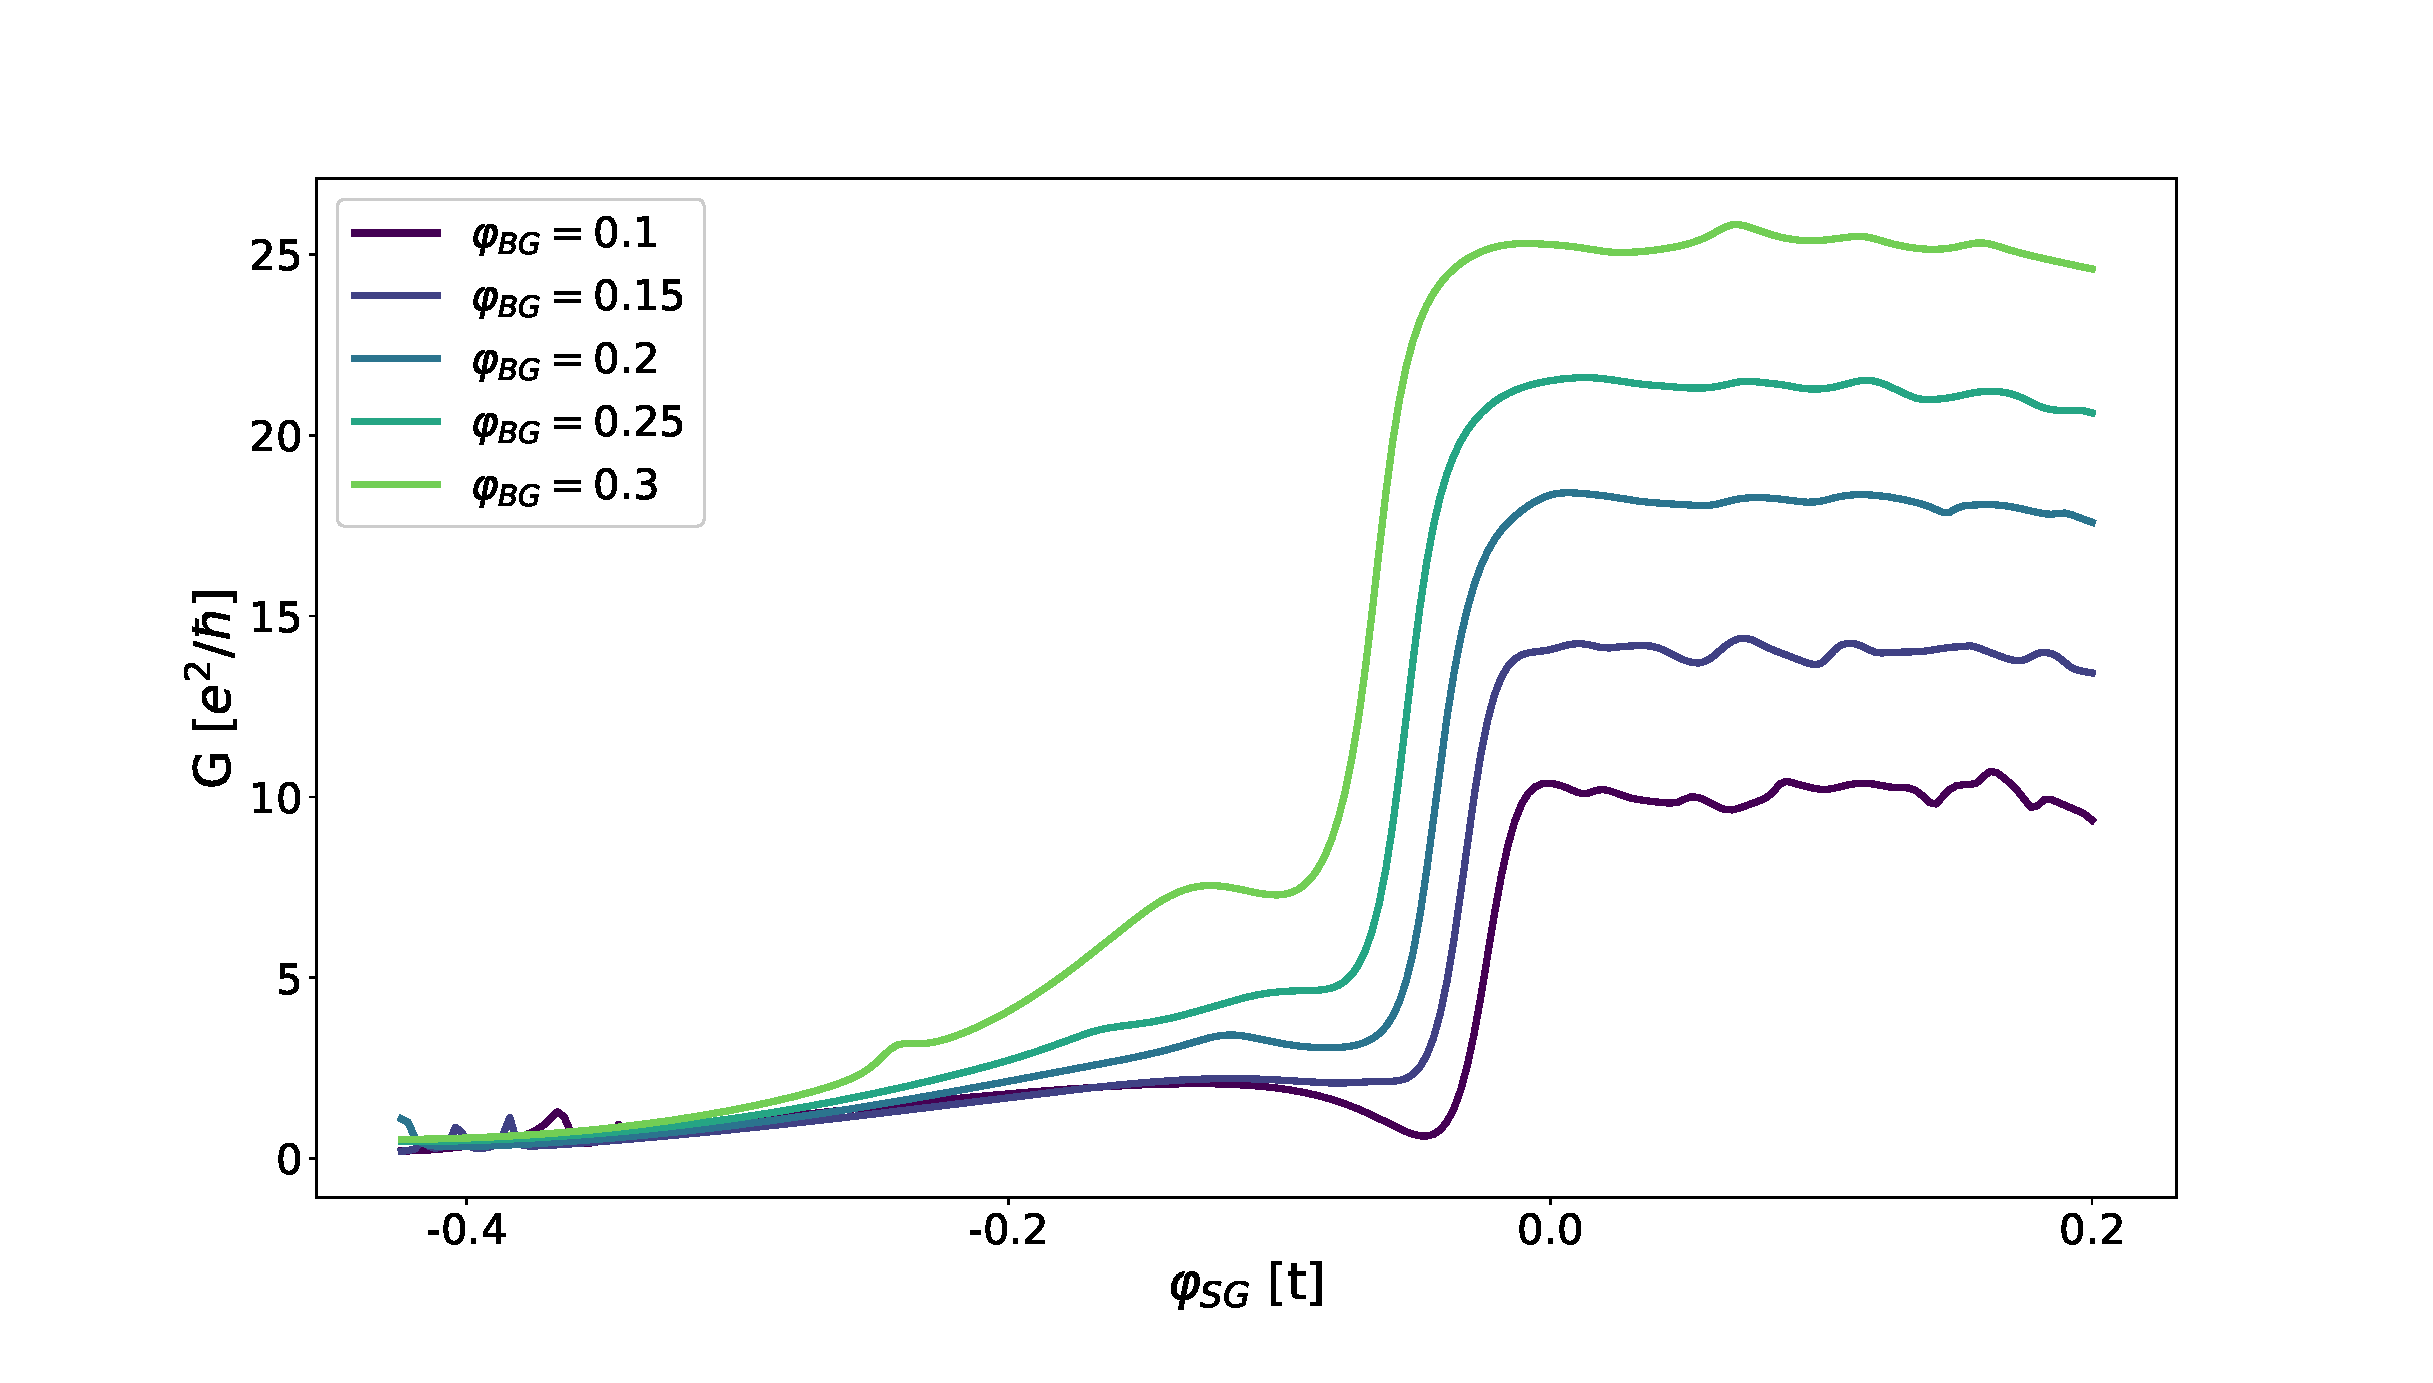
\includegraphics[width=\textwidth]{figure/numericalmodel/qpc-conductance}
\caption{Conductance QPC} \label{fig:qpc-conductance}
\end{minipage}
%\hspace{0.5cm}
\begin{minipage}[b]{0.49\linewidth}
\centering
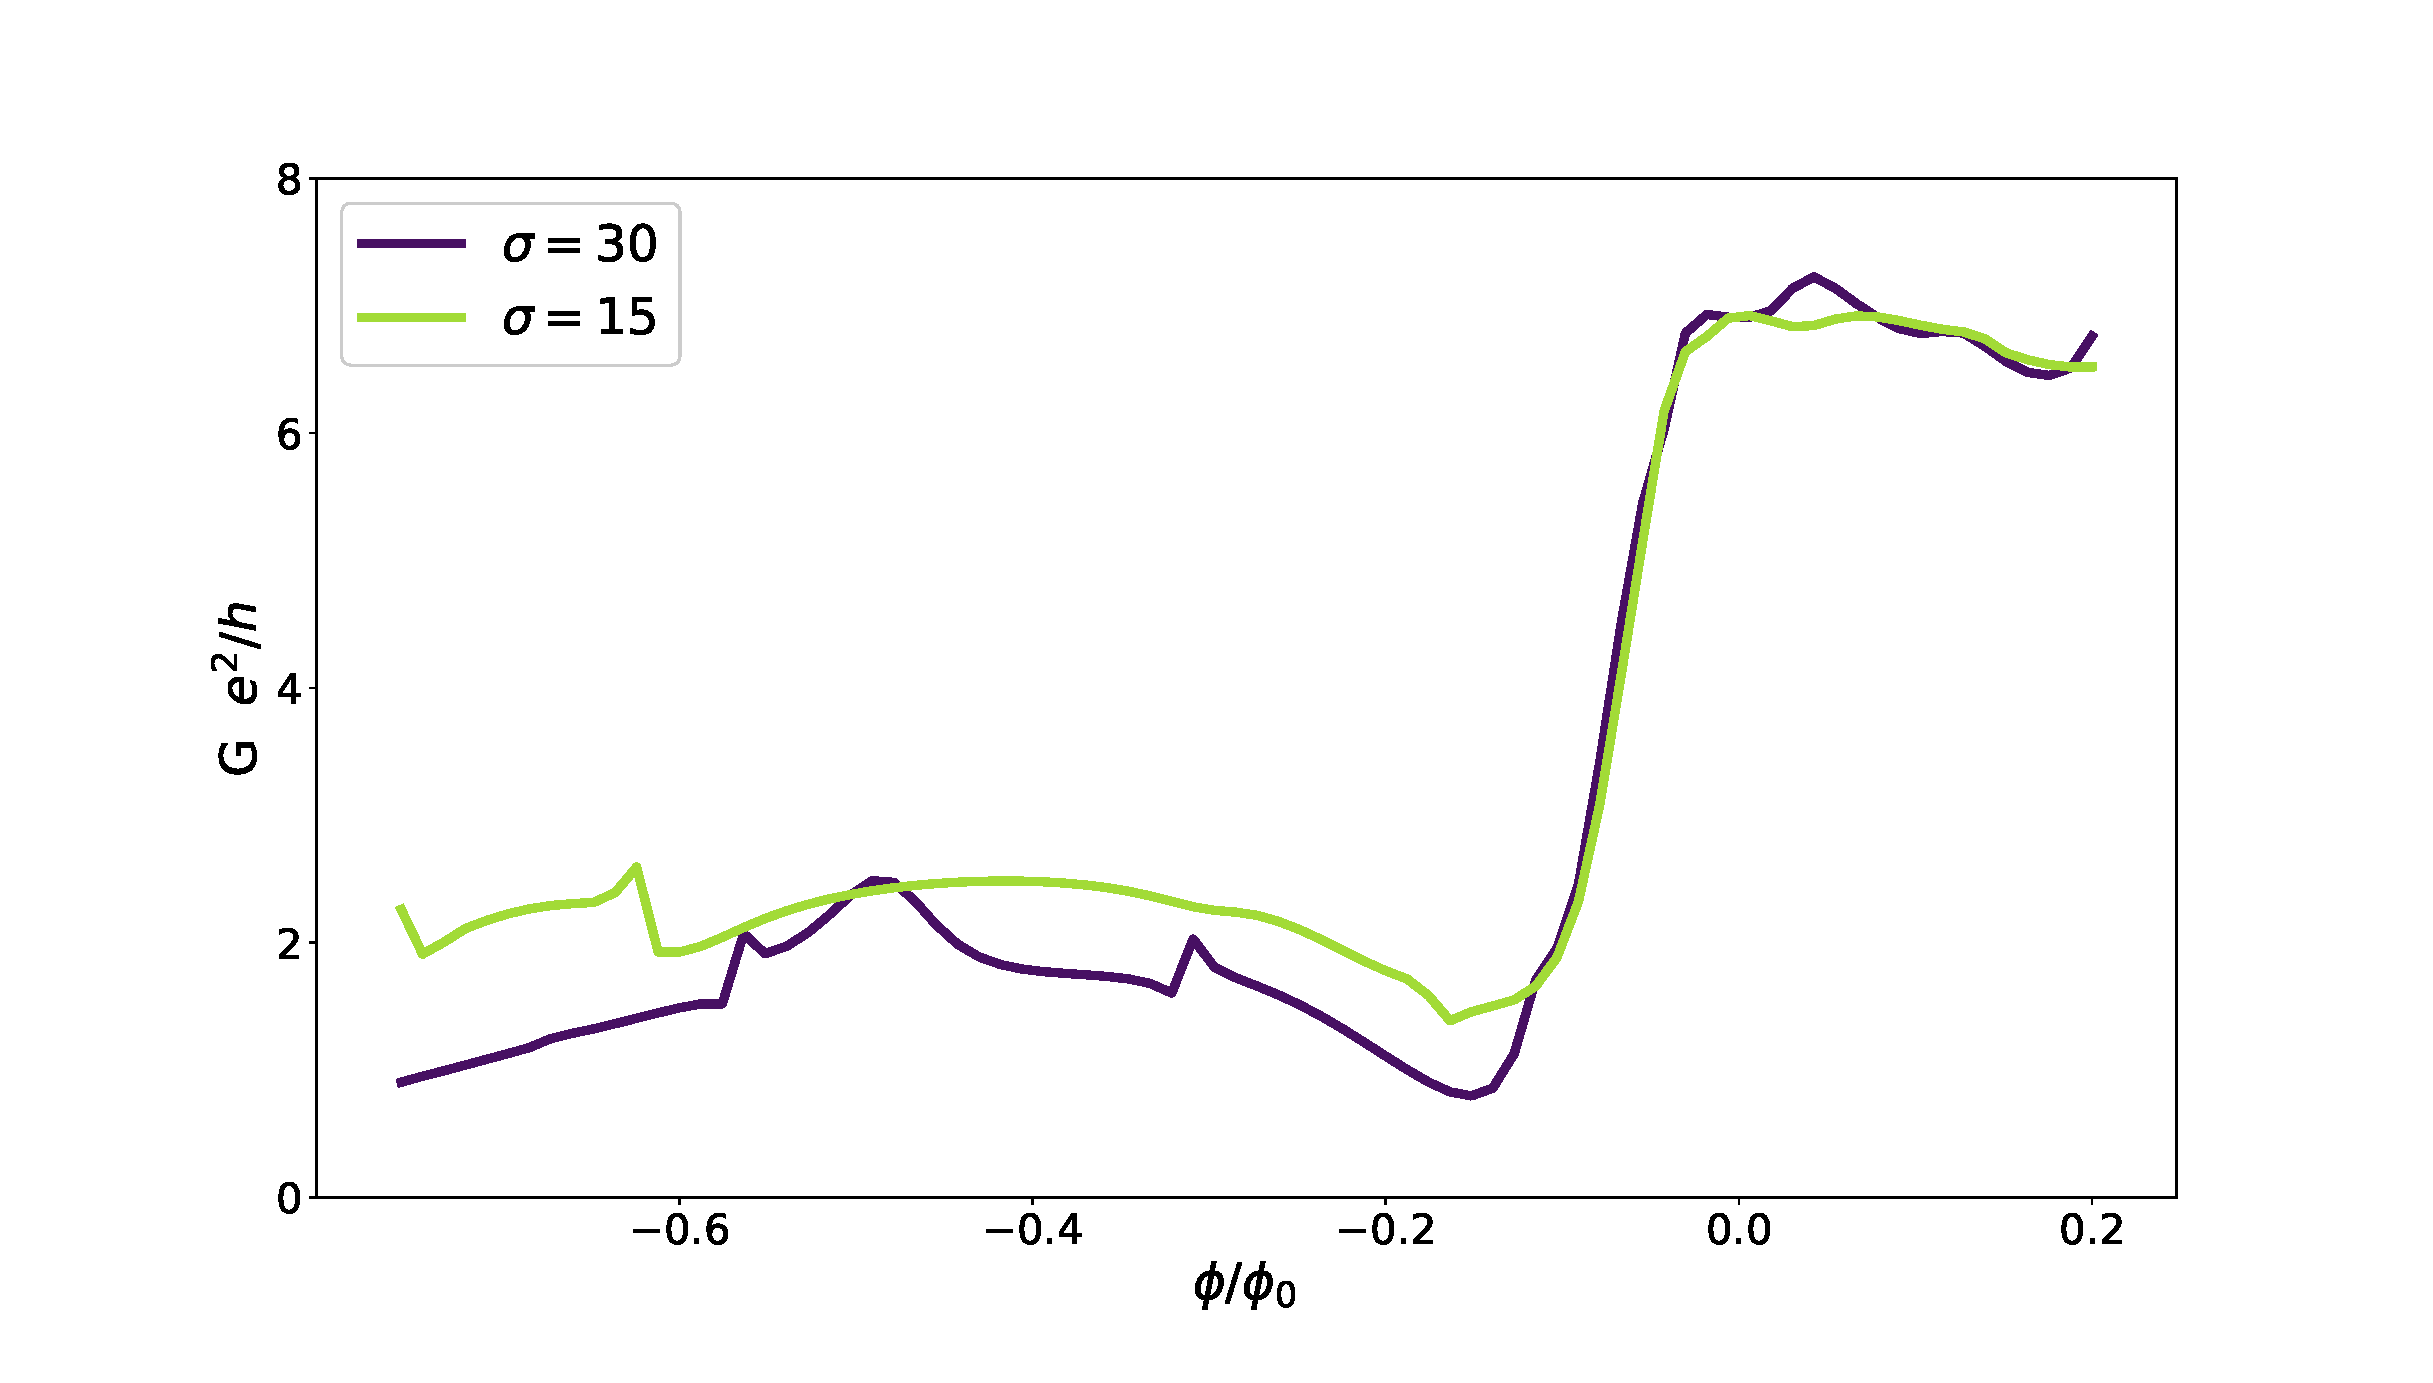
\includegraphics[width=\textwidth]{figure/numericalmodel/conductance-sigma}
\caption{default}\label{fig:qpc-conductance-sigma}
\end{minipage}
\end{figure}

A fixed back-gate voltage leading to an n-doping of the scattering region is assumed, because the measurements of the experiment where conducted at fairly low charge carrier density. For increasingly negative values of the split-gate voltage, the region underneath the top gate becomes p-doped. The higher the split-gate voltage, the lower the transparency of the barrier becomes, and at a certain point, the current transport is confined to very few channels (see section \ref{sec:exp-normal-state}). In figure \ref{fig:qpc-conductance}, the conductance is plotted versus split-gate voltage. For increasingly negative values of the split-gate voltage, only few conducting channels remain. For the following calculations the back-gate voltage is chosen to be $\varphi_{BG} = 0.2$.

For increasingly positive back-gate voltage, the overall conductivity of the sample increases and the critical current cannot be confined.

The stray fields produced at the edges of the top-gate voltage are being considered as well since they are crucial for the conductive behaviour of the barrier. They are modelled as a gaussian filter applied to the vertical electric field lines:
\begin{equation}
g (x) = \frac{1}{\sqrt{2 \pi} \sigma} e^{-\frac{x^2}{2 \sigma ^2}}.
\end{equation}

Figure \ref{fig:qpc-conductance-sigma} shows two conductance lines for the same back-gate of $\varphi_{BG} = 0.2$, differing only in their $\sigma$ values. For very high values of $\sigma$, the QPC stops to function as a confinement of the current, but becomes an entirely reflective barrier. For $\sigma = 30$, the conductance falls below the threshold of 1.

\begin{figure}[h]
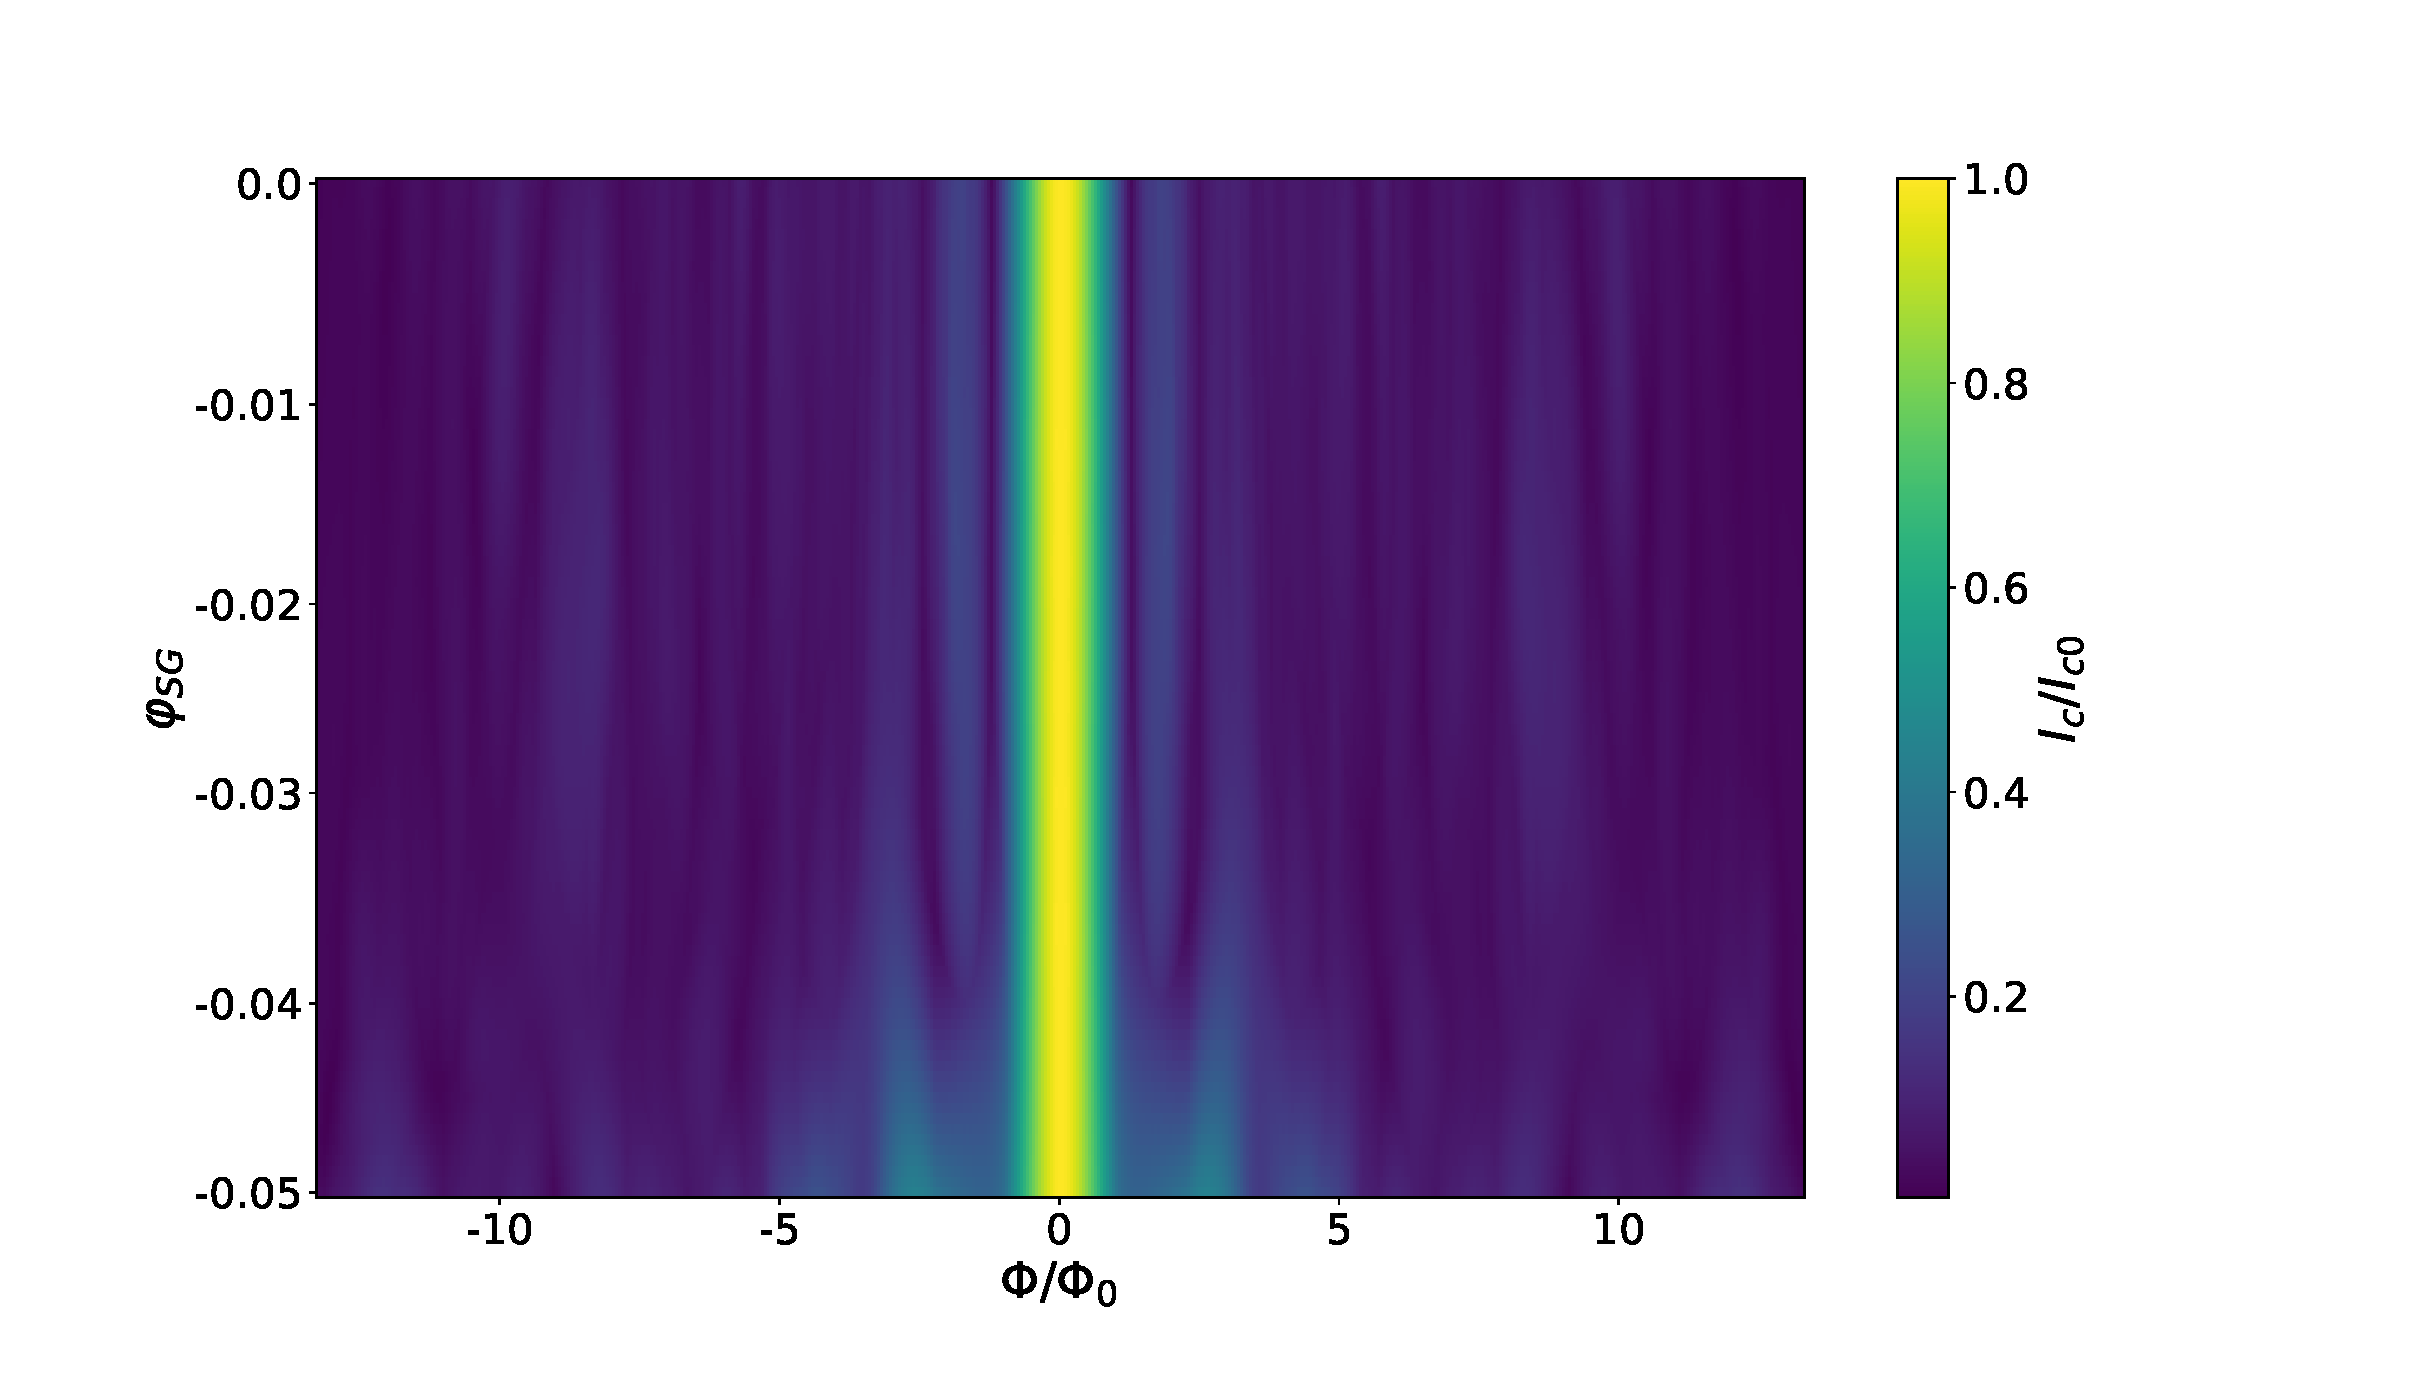
\includegraphics[width=\textwidth]{figure/numericalmodel/qpc_icnorm_heatmap}
\caption{The normed critical current $I_c^\text{norm}$ as a function of quantised flux and split-gate voltage $\varphi_{SG}$. }\label{fig:qpc-heatmap}
\end{figure}

Figure \ref{fig:qpc-heatmap} shows the the supercurrent that has been simulated by the procedure presented in \ref{sec:scattering-supercurrent}. The normed critical current is displayed as the heat color. It is plotted against the normed flux for different split-gate potentials. One can see clearly that for a split-gate potential of approximately 0 -- a transmissive barrier -- the critical current has the form of a Fraunhofer-like beating pattern. With increasing split-gate potential, the barrier becomes increasingly reflective, a constriction is formed, and the current is confined. A bell-shaped pattern is observed. This corresponds well to the findings presented in \ref{ch:experiment}. It should be noted that the transition from beating pattern to bell-shaped pattern happens on a narrow range of the split-gate potential.

\section{Half-Barrier}
The two fingers of the QPC experiment can be tuned individually, so measurements of individually gated (half-barrier) set-ups  were included in the experimental set-up. As of yet, no measurement data has been published, though.

The simulations have been carried out with a higher back-gate potential, which explains the higher values of the split-gate potential in the following plots. It is not important to have a low charge-carrier density, because this set-up does not aim to confine the current. A back-gate potential of as high as $\varphi_{BG} = 0.8$ has been chosen.

The plot in figure \ref{fig:hb-abs} shows that when the barrier is fully formed, $I_{c0}$ is halved compared to its value when there is no split-gate. Figure \ref{fig:hb-norm} illustrates that as the barrier forms, the periodicity of the pattern almost doubles. This behaviour is observed in the experiment as well.

The halving of the critical current peak can be explained within the framework of the quasi-classical theory. When a barrier is fully present, only half of the trajectories connecting the superconnecting leads can pass. The asymmetry of the sample 
%Half barrier calculation for $\varphi_{BG} = 0.8$. Hier sieht man eine Verdopplung der Periode. Ergibt ja auch Sinn, weil wenn nämlich die Barriere aufgebaut wird, ändert sich die Fläche, die effektiv zur Verfügung steht. Und wenn sich die effektive Fläche ändert, ändert sich auch die Phase. Die sind nämlich über komplizierte Relationen verknüpft, die ich alle schon mal hergeleitet habe.
%Tatsächlich spiegelt sich in diesem Setup auch die Asymmetrie wieder: Je nachdem welcher Finger (der obere oder der untere) angeschaltet ist, verändert sich das Maximum des kritischen Stroms weil da nämlich entweder mehr oder weniger Trajektorien durchkommen. Macht Sinn, ne?
%\begin{figure}[h]
%\includegraphics[width=\textwidth]{figure/numericalmodel/}
%\caption{qpc conductance}\label{fig:half-barrier}
%\end{figure}

\begin{figure}[ht]
\begin{minipage}[b]{0.49\linewidth}
\centering
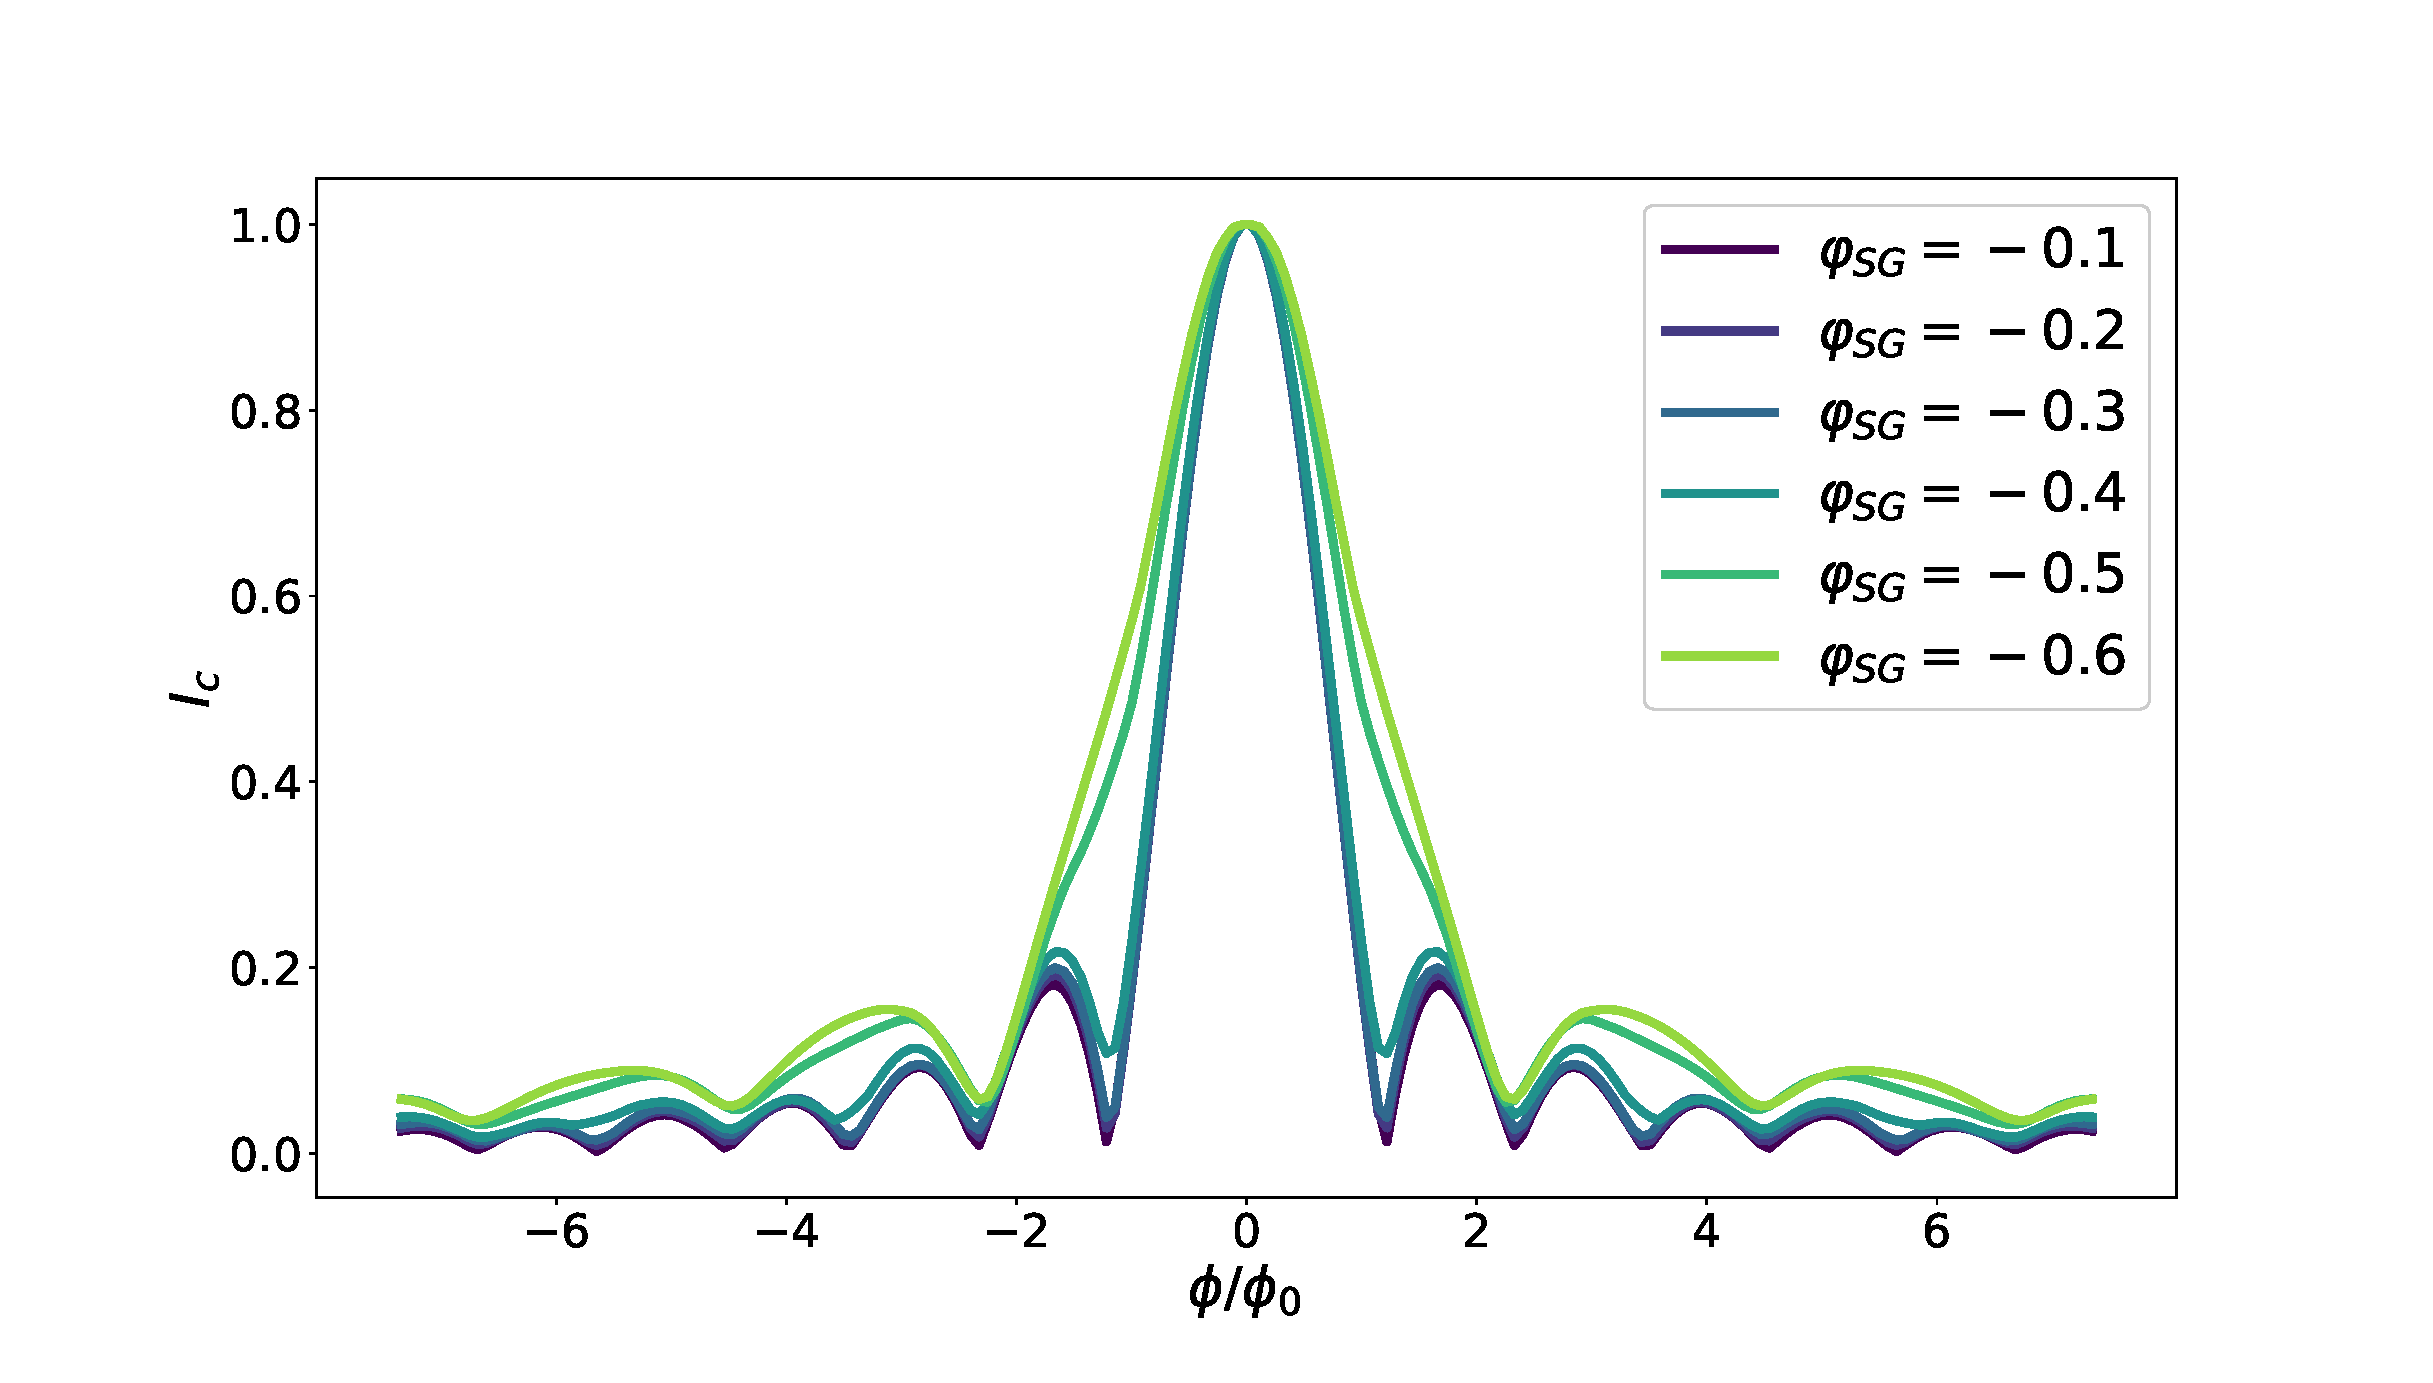
\includegraphics[width=\textwidth]{figure/numericalmodel/hb_upper}
\caption{HB normalized current } \label{fig:hb-norm}
\end{minipage}
%\hspace{0.5cm}
\begin{minipage}[b]{0.49\linewidth}
\centering
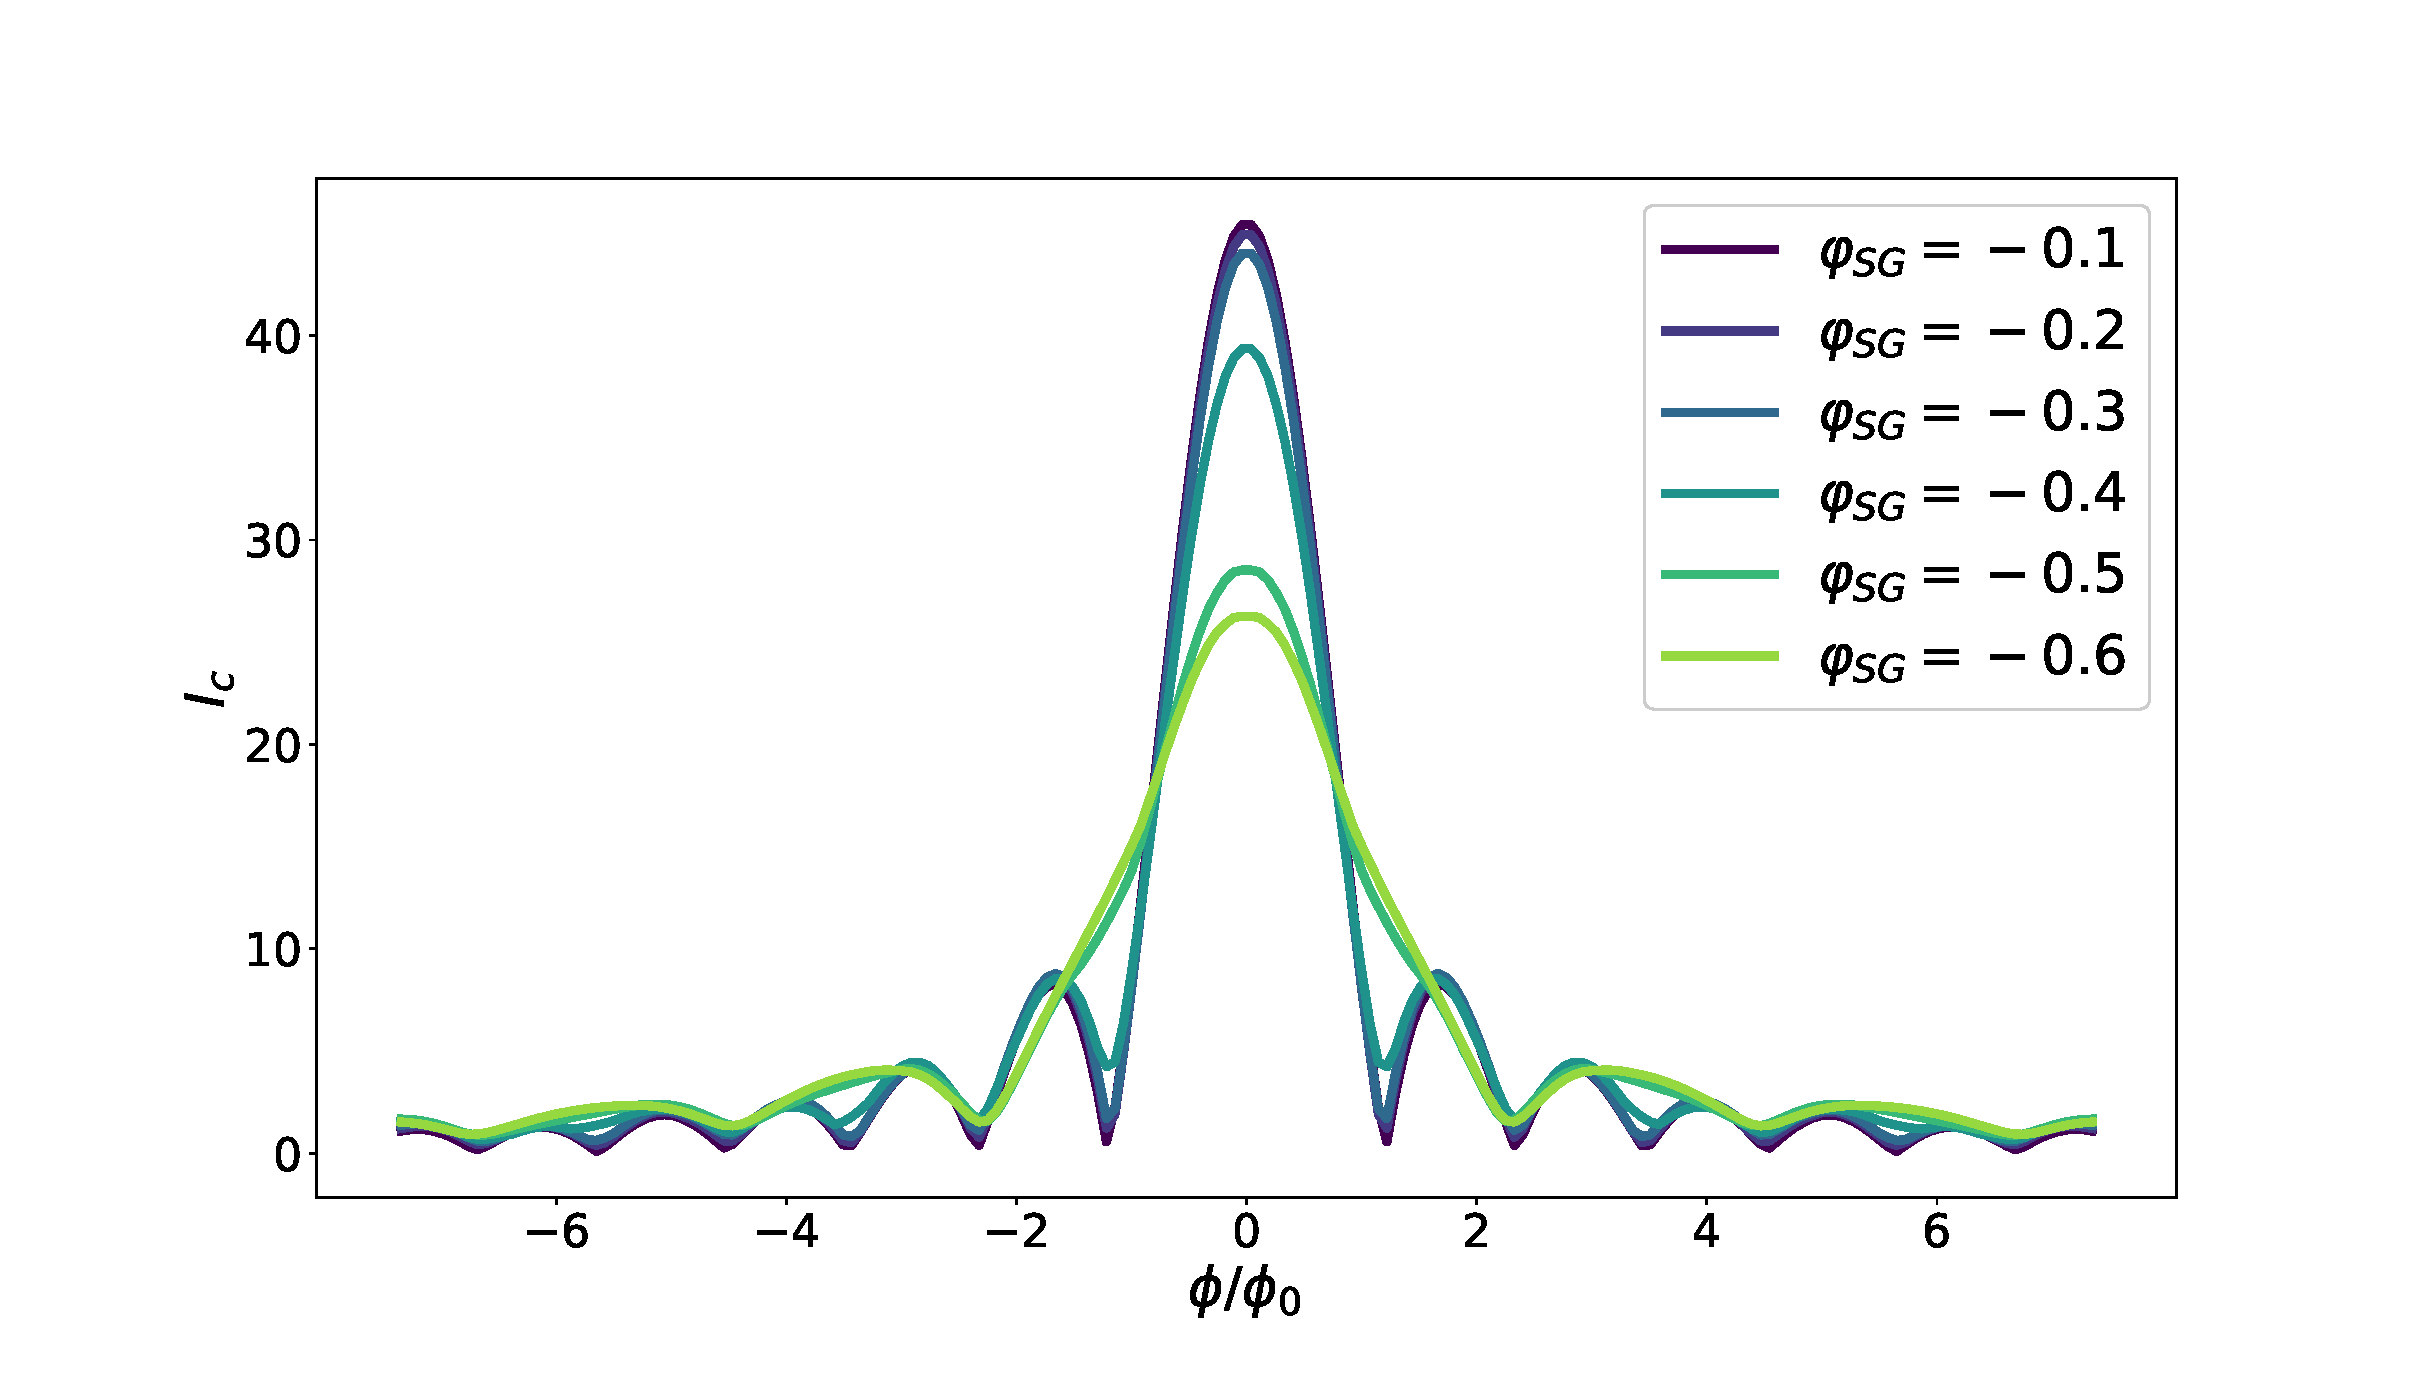
\includegraphics[width=\textwidth]{figure/numericalmodel/hb_upper_abs}
\caption{HB current}\label{fig:hb-abs}
\end{minipage}
\end{figure}

%Ergebnis: Die Periode verändert sich, mit der Fläche, die Asymmetrie spielt eine Rolle.

\section{Waveguide}
%Waveguide 3, 2 for $\varphi_{BG} = 0.5$ 
%Waveguide ist spannend, weil: symmetrie in die x Richtung sorgt dafür, dass man den Strom Fourier transformieren kann. Das geht mit der Methode von Dynes and Fulton \cite{Dynes1971}

\begin{figure}[ht]
\begin{minipage}[b]{0.5\linewidth}
\centering
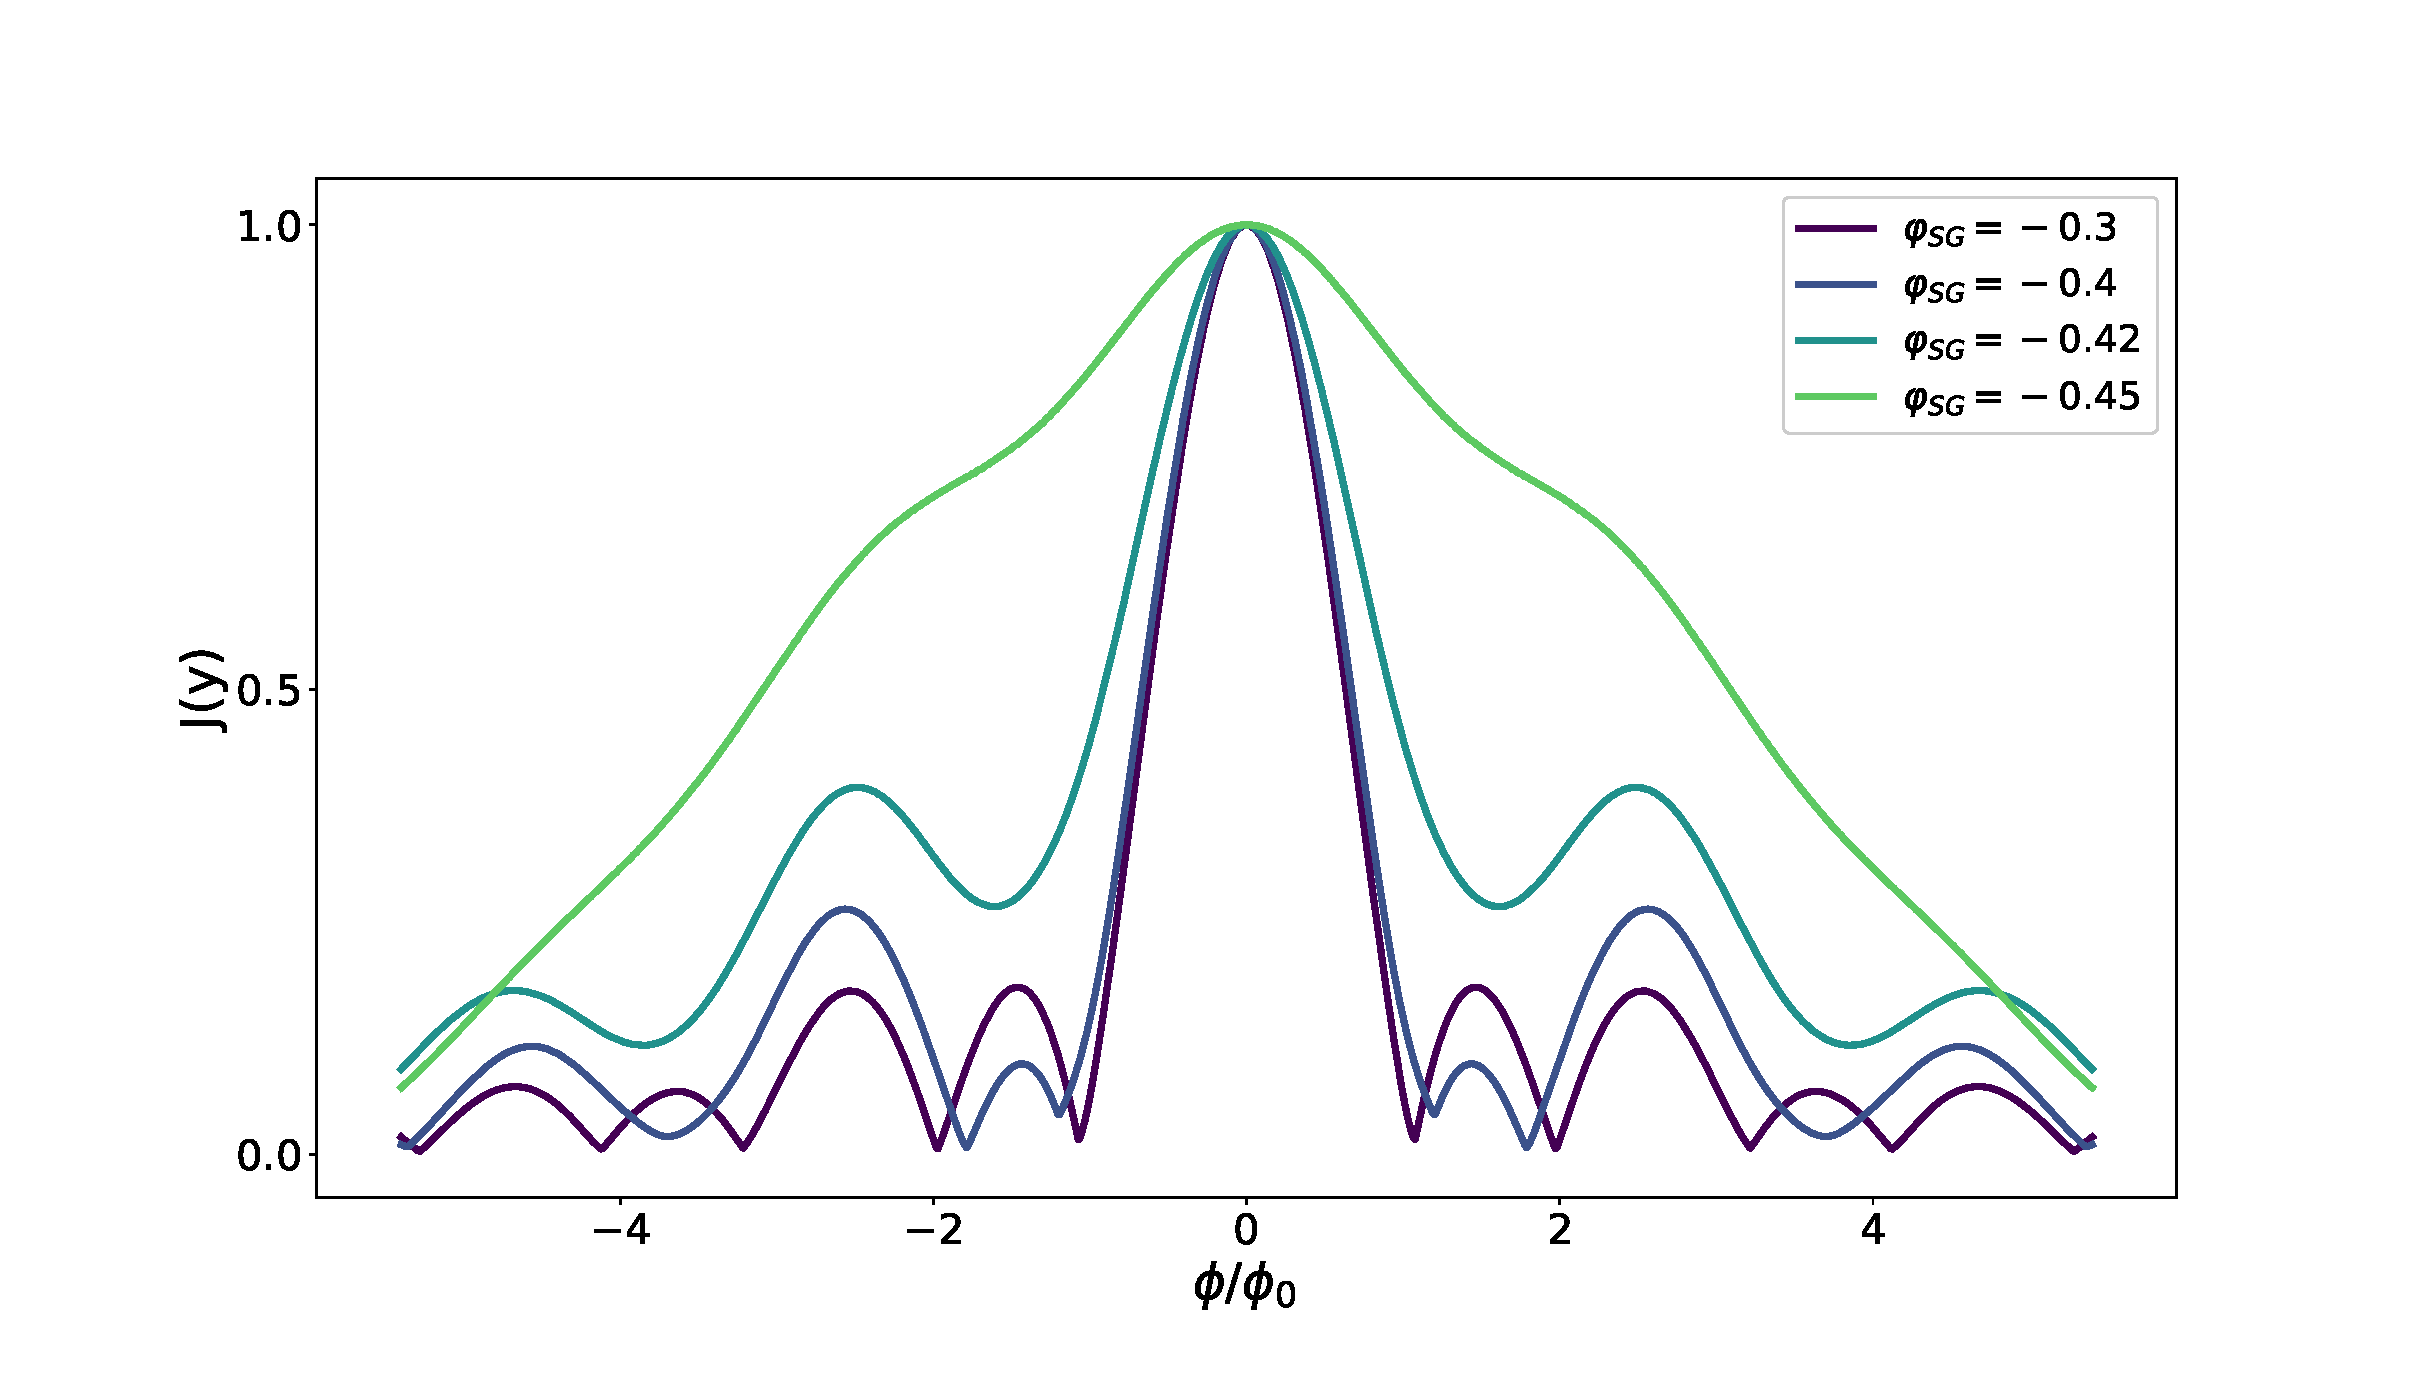
\includegraphics[width=\textwidth]{figure/numericalmodel/waveguide-ic}
\caption{Conductance QPC} \label{fig:qpc-conductance}
\end{minipage}
%\hspace{0.5cm}
\begin{minipage}[b]{0.5\linewidth}
\centering
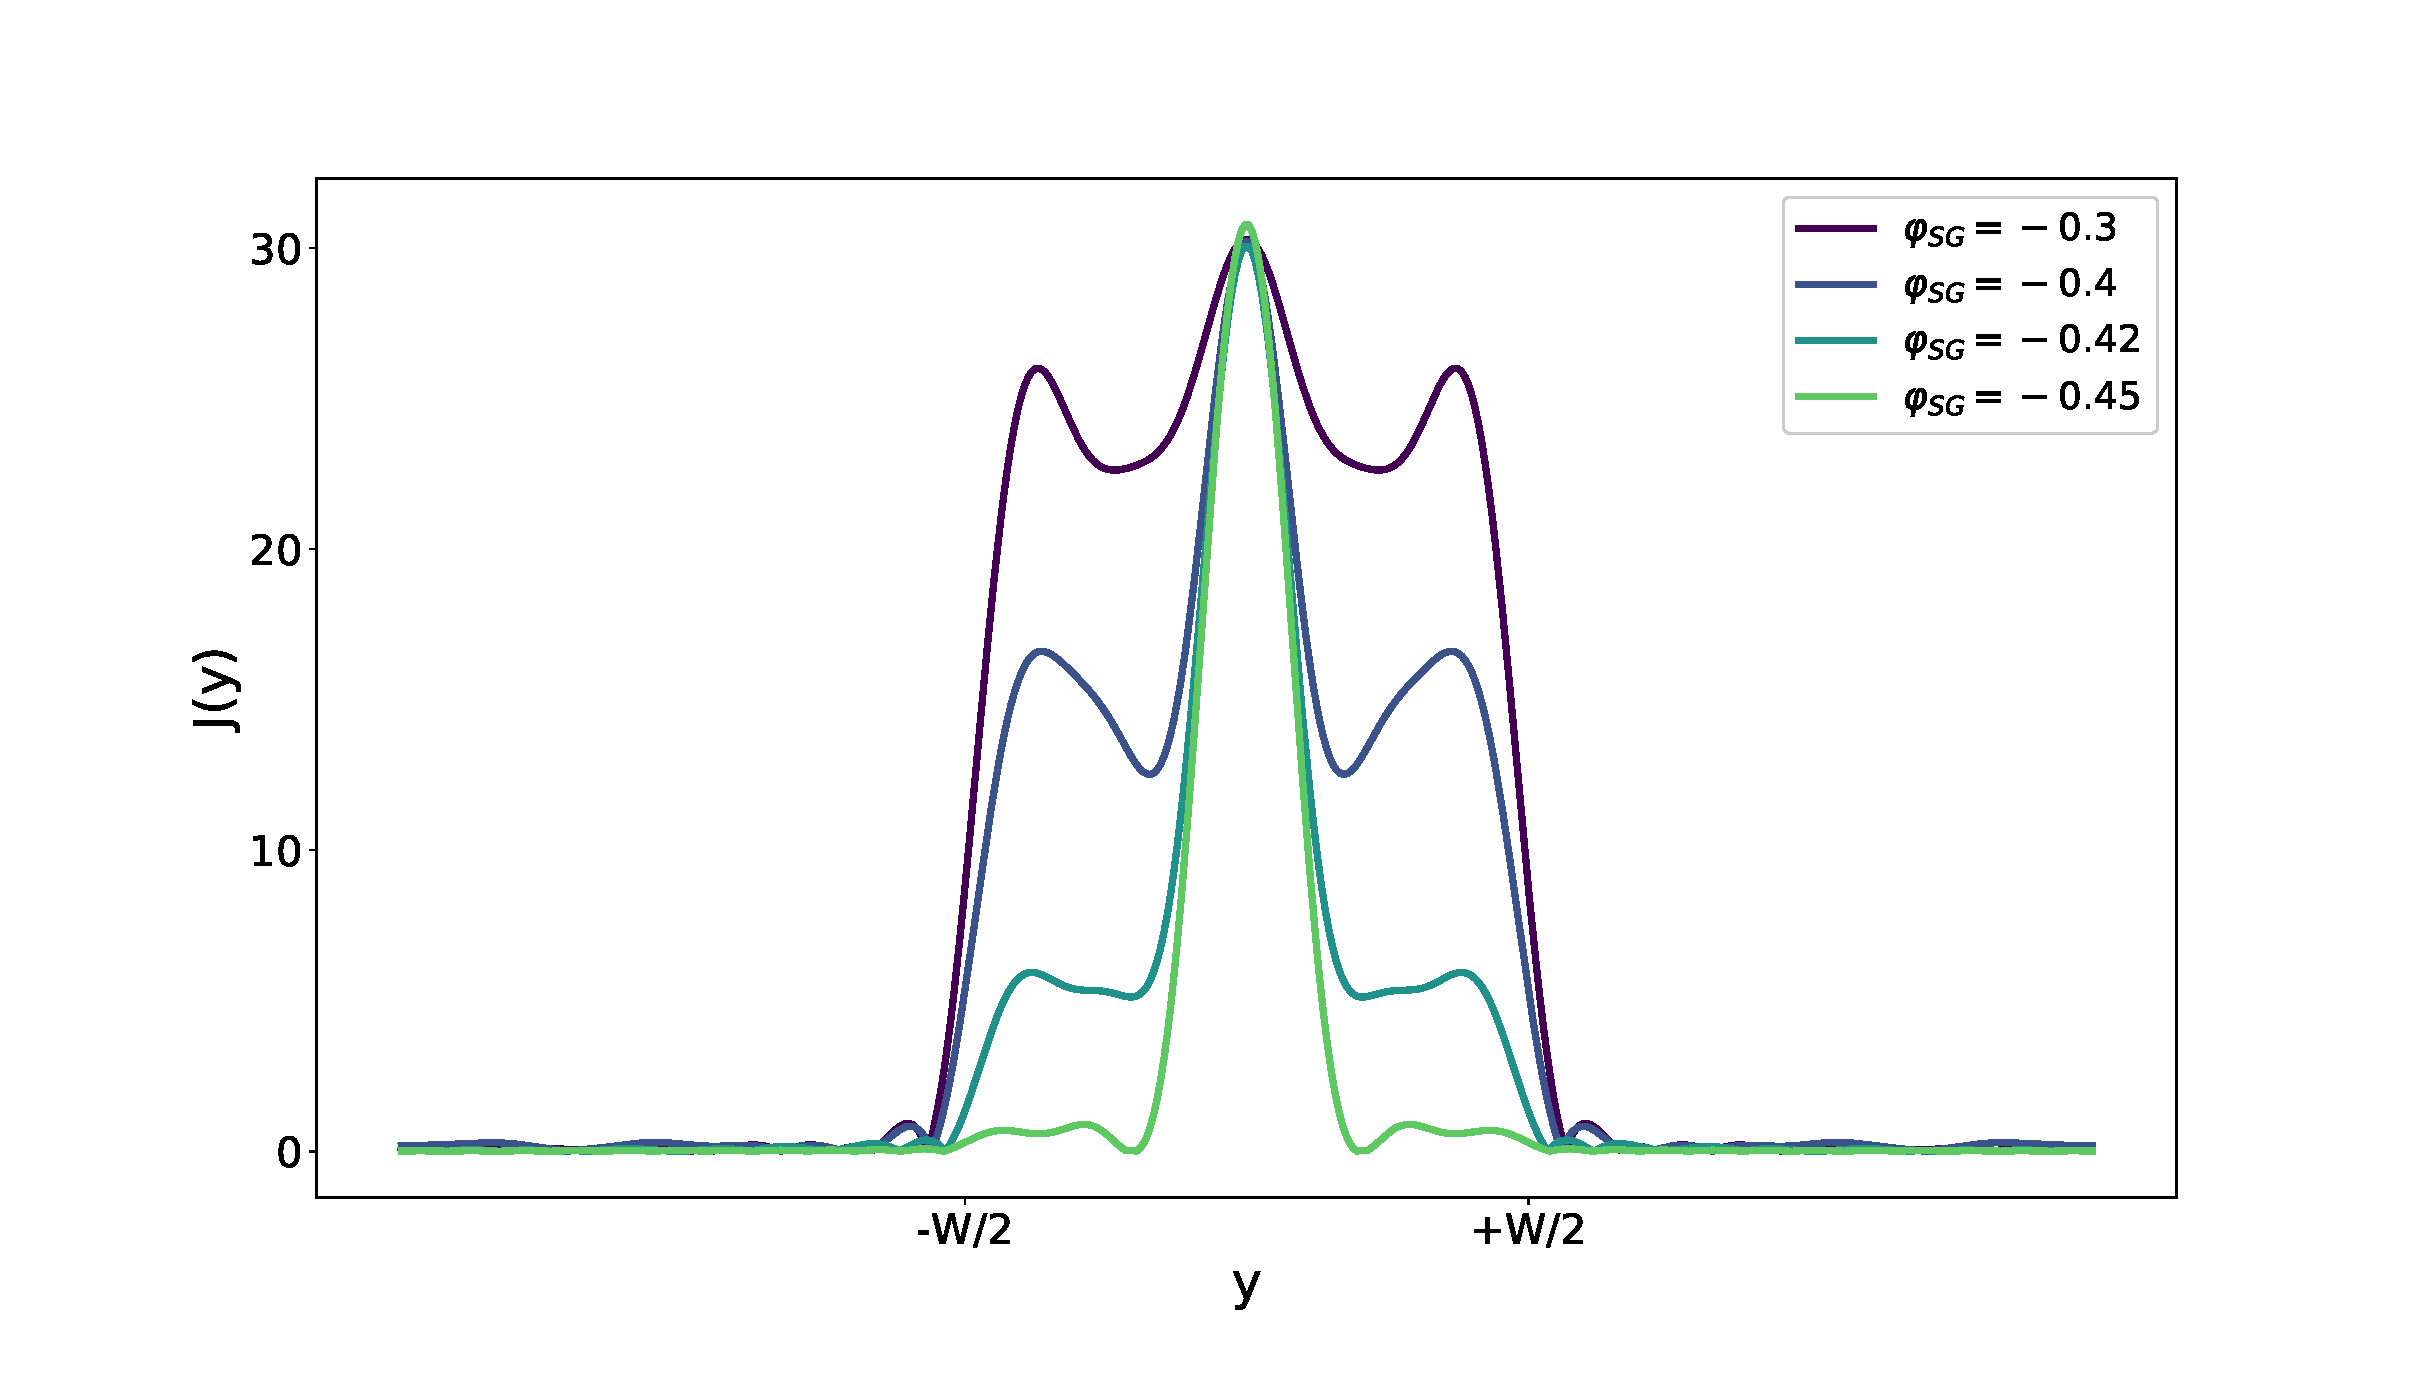
\includegraphics[width=\textwidth]{figure/numericalmodel/waveguide-jy}
\caption{default}\label{fig:qpc-conductance-sigma}
\end{minipage}
\end{figure}

%Ergebnis: Strom wird eingeschränkt auf wenige Channels